%!Tex Root = ../Tutorat3.tex
% ./Packete.tex
% ./Design.tex
% ./Deklarationen.tex
% ./Aufgabe2.tex
% ./Aufgabe3.tex
% ./Aufgabe4.tex
% ./Bonus.tex

\section{Task 1}

\setcounter{task}{1}

\begin{frame}{Task 1}{Earliest Deadline Due}
  \begin{requirements}
    \begin{itemize}
      \item \alert{non-preemptive}
      \item tasks have \alert{same arrival times} (synchronous arrivals)
      \item $min(D_i)$ for all remaining $J_i$
      \item \alert{minimizing} the \alert{maximum lateness}
      \item tasks are \alert{independent}
    \end{itemize}
    \centering
  \end{requirements}
  \centering
  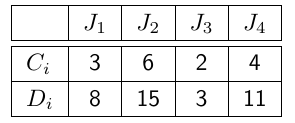
\includegraphics[height=0.2\paperheight]{./figures/1_tab.png}
  ($\forall J_i: r_i = 0$)
\end{frame}

\begin{frame}{Task 1}{Earliest Deadline Due}
  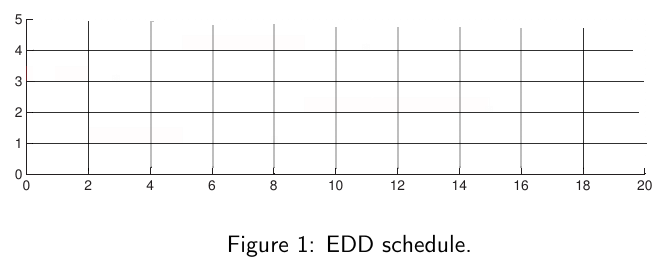
\includegraphics[width=\textwidth]{./figures/1_empty.png}
\end{frame}

\begin{frame}{Task 1}{Earliest Deadline Due}
  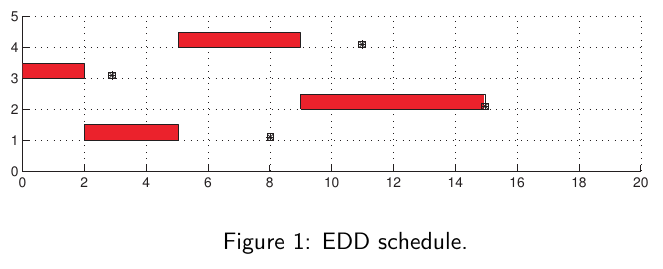
\includegraphics[width=\textwidth]{./figures/1_sol.png}
\end{frame}
